%!TEX root = ../documentation.tex

\chapter{Grundlegende Komponenten und deren Funktionsweise}
Norbert hat zur Aufgabe Informationen / Daten innerhalb eines Kurses zu teilen.
Jeder Benutzer hat einen Newsfeed in dem diese Informationen angezeigt werden.
Die Informationen werden von Newsfeeds der Benutzer und externen Diensten ermittelt.
Anschließend muss es eine zentrale Logik geben, die diese \enquote{Daten} klassifiziert und den 
Benutzern neue Daten vorschlägt. (Siehe Abbildung \ref{overview:general-function})

\begin{figure}[H]
    \centering
    \includegraphics[width=0.9\textwidth]{images/Allgemeine-Funktionsweise.png}
    \caption{Funktionsweise des Newsfeeds}\label{overview:general-function}
\end{figure}

Eine grundlegende Anforderung dafür ist das sammeln von Daten.
Diese können durch Studenten oder externe Dienste angelegt werden.

Diese Daten werden wenn sie von einem Benutzer erstellt wurden als Einträge bezeichnet 
und wenn sie von einem externen Dienst angelegt wurden als Informationen bezeichent.

Bei Verwendung der Anwendung werden dem Benutzer seine Einträge angezeigt.

Jetzt hat der Benuter die Möglichkeit neue Einträge zu erstellen und hinzuzufügen,
oder er bekommt durch die Anwendung neue Einträge vorgeschlagen, welche im folgenden als Vorschlag bezeichnet werden.

Die Daten von einem externen Dienst werden als Information gespeichert und den Benutzern angezeigt.

Es gibt also insgesamt 3 verschiedene Arten von Daten mit denen ein Benutzer interagiert welche in Tabelle \ref{overview:newsfeedelement}
zu sehen sind.

\begin{table}[H]
    \centering
    \begin{tabularx}{\textwidth}{|X|X|X|}
            \toprule
            \textbf{Eintrag} & \textbf{Vorschlag} & \textbf{Information} \\
            \midrule
            \endhead
            Ein Eintrag dient zum notieren von Daten. Er kann mehrere Eigenschaften haben, wie z.B. eine Erinnerung.
            Ein Eintrag kann von einem Benutzer bearbeitet werden.
            &
            Die Anwendung analysiert ständig die Einträge aller Benutzer. Wenn erkannt wird, dass sich ein Benutzer
            für einen Eintrag eines anderen Benutzers interessieren könnte wird ihm dieser als \enquote{Vorschlag} vorgeschlagen.
            &
            Wenn durch einen externen Dienst Daten produziert werden, wie z.B. eine E-Mail an den Kursverteiler versendet wird,
            werden diese Daten als \enquote{Information} allen Benutzern vorgeschlagen.
            Der Benutzer hat dann die Möglichkeit diese Informationen zu auszublenden, wenn er sich nicht dafür interessiert.
            \\
            \hline
    \end{tabularx}
    \caption{Elemente des Newsfeeds}\label{overview:newsfeedelement}
\end{table}

Da Benutzer nicht immer eine Verbindung zu der Anwendung haben wird für die Architektur eine Client-Server Architektur gewählt.
Dadurch können Daten zentral auf einem Server gesammelt bzw. klassifiziert werden und anschließend an die Clients verteilt werden.
Diese Architektur hat den Vorteil, dass die Daten zentral ausgewertet werden können.

Folgende Funktionalitäten müssen von der Architektur zwingend erfüllt werden, damit Norbert korrekt funktionieren kann:
\begin{enumerate}
	\item Der Newsfeed muss auf dem Client angezeigt werden können.
	\item Norbert muss die gesamten Daten (Einträge, Vorschläge, E-Mails. etc.) zentral speichern.
	\item Die für den Newsfeeds relevanten Daten müssen von Norbert an die Clients geliefert werden können.
	\item Der Client muss Einträge anlegen/bearbeiten können und auf Vorschläge reagieren können, bzw. seine Aktionen Norbert mitteilen können.
	\item Norbert muss ToDo-Vorschläge liefern können.
\end{enumerate}


\section[Grundlegender Aufbau]{Grundlegender Aufbau aus Funktionssicht}


  Die in Grafik \ref{fig: Overview_HLVL} gezeigte Architektur würde die oben genannten Kriterien erfüllen.
  \begin{enumerate}
  	\item Über einen Webbrowser kann der Newsfeed auf den Clients angezeigt werden.
  	\item Norbert hat die gesamten Daten in getrennten Dateien/Ordnern zur Verfügung.
  	\item Über die Kommunikationsschnittstelle kann Norbert die relevanten Daten an den Client liefern.
  	\item Über die Kommunikationsschnittstelle können die Aktionen der Clients Norbert mitgeteilt werden.
  	\item Die Vorschlagslogik berechnet anhand der vorhandenen Daten Vorschläge, welche über die Kommunikationsschnittstelle an den Client geliefert werden.
  	\end{enumerate}

  	
\begin{figure}[H]
\centering
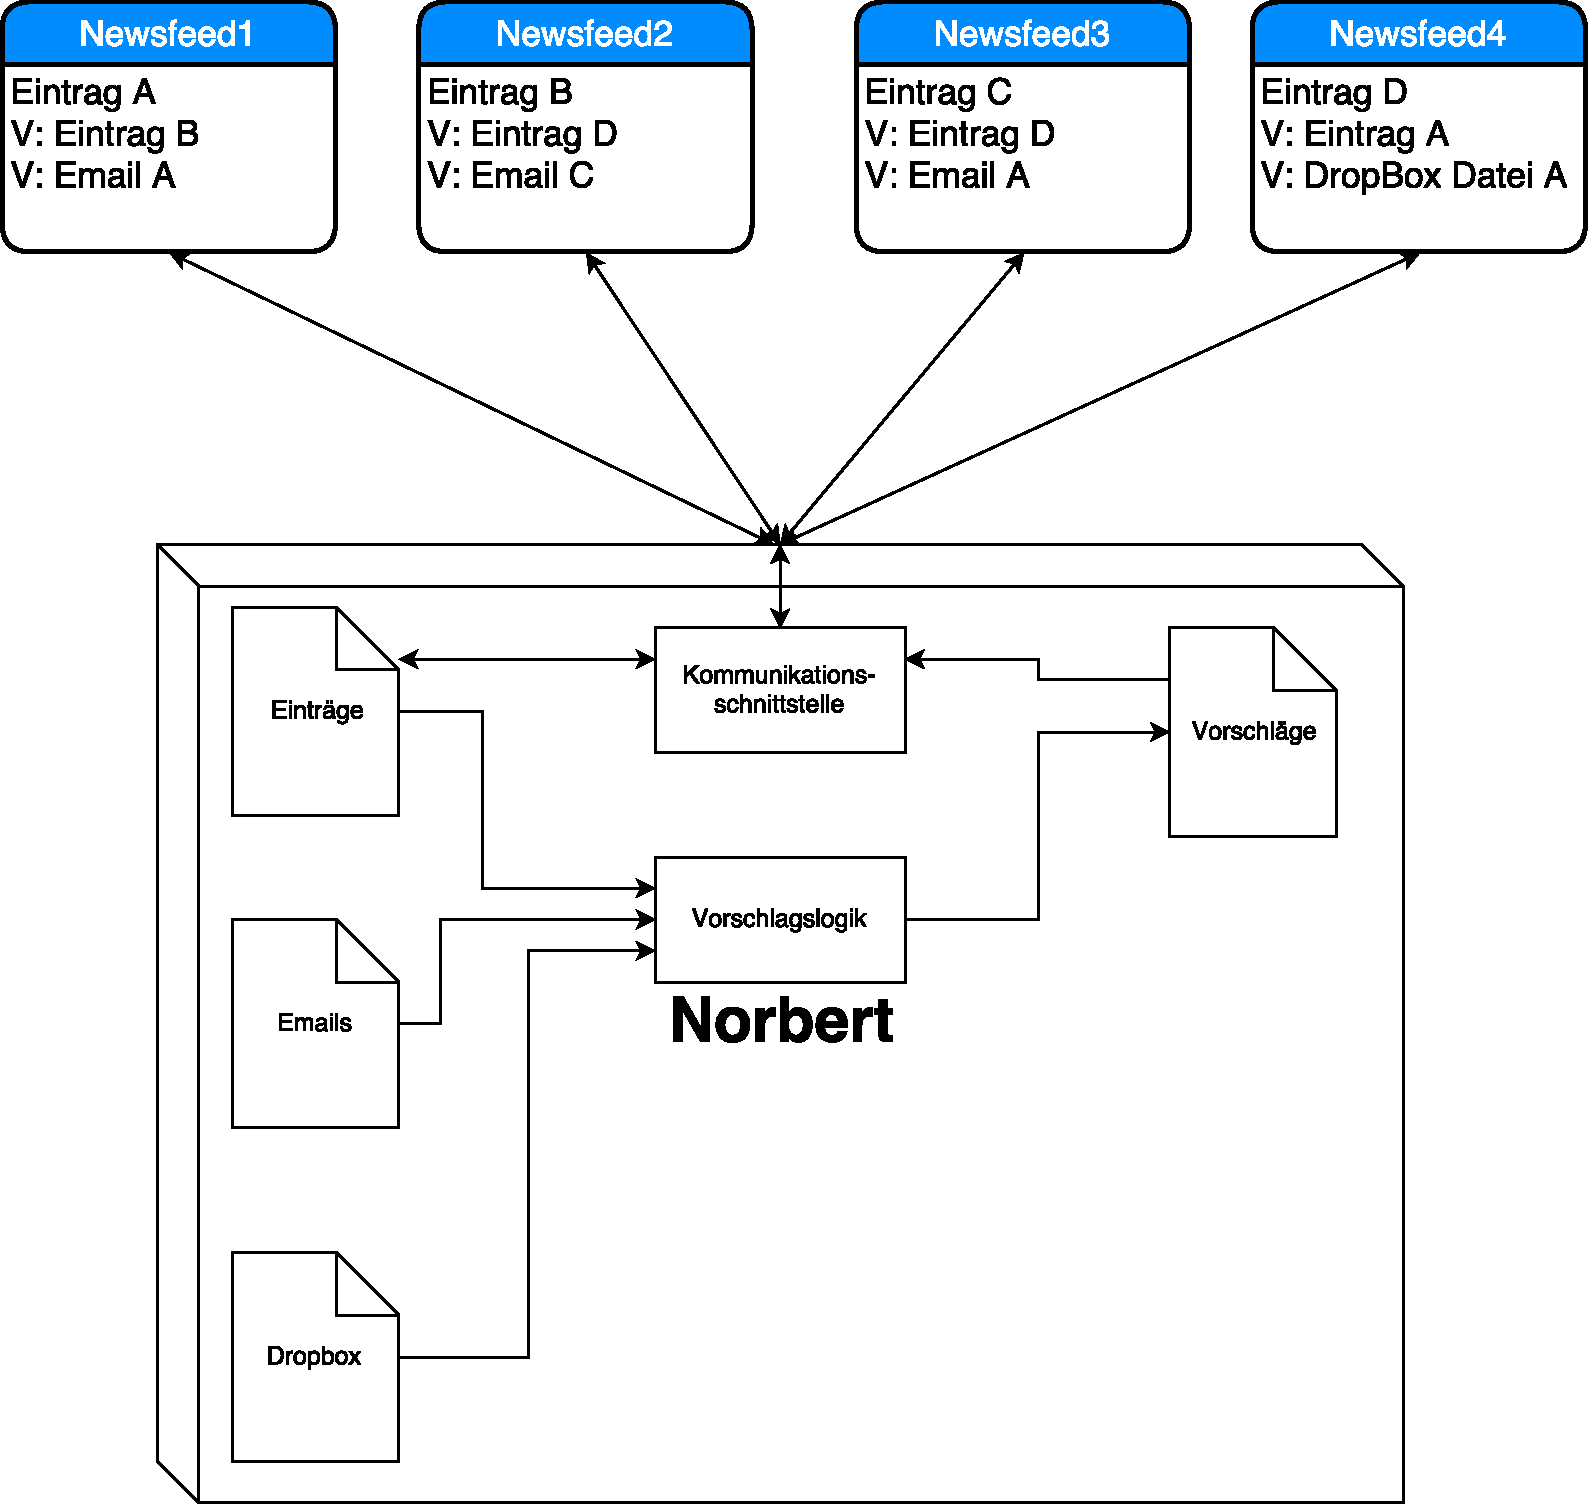
\includegraphics[scale=0.6]{uml-diagramms/overview_hlvl.pdf}
\caption{Grundlegende Funktionalität}
\label{fig: Overview_HLVL}
\end{figure}

Mit dieser Architektur treten aber mehrere Probleme auf:
  	\begin{enumerate}
  	\item Das manuelle Verwalten von Daten in separaten Dateien ist sehr aufwendig und extremst fehleranfällig.
  	\item Der Ablauf interner Prozesse ist nicht definiert und es ist unklar, wie dieser gesteuert wird
  	\end{enumerate}

\section{Datenhaltung}

Das erste Problem kann durch die Verwendung eines Datenbanksystems gelöst werden. Durch eine Datenbank können die Daten zentral verfügbar gemacht werden. Außerdem ist der Zugriff über ein Datenbanksystem weniger fehleranfällig und in der Regel auch effizienter, da die meisten Datenbanksysteme bereits von Haus aus Performanceoptimierungen wie Puffer etc. mitbringen. 
\begin{figure}[H]
\centering
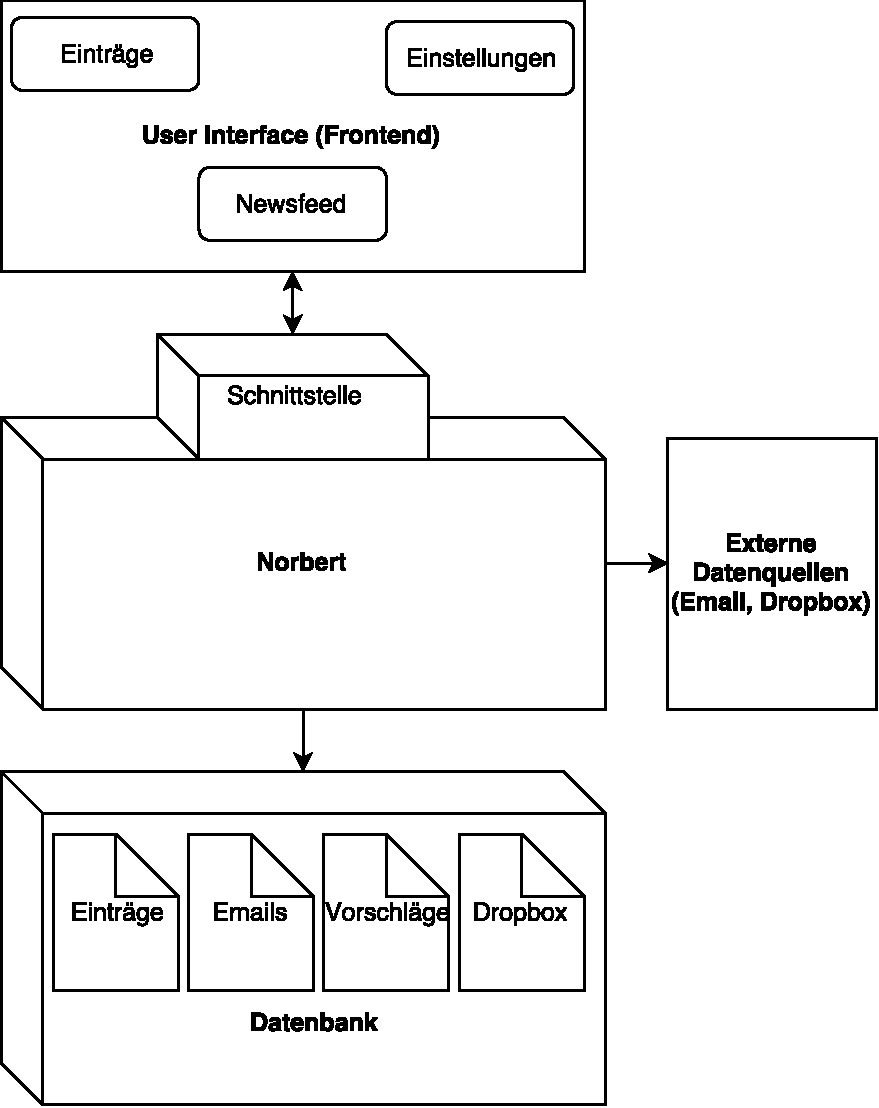
\includegraphics[scale=0.75]{uml-diagramms/daten_hlvl.pdf}
\caption{Kapselung der Daten in einer Datenbank}
\label{fig: DB_HLVL}
\end{figure}

\section{Interne Prozesse}

Das zweite Problem kann durch eine Komponente zur Aufgabenverwaltung gelöst werden. Anstatt alle Aufgaben in Echtzeit zu bearbeiten, werden bestimmte Aufgaben, die besonders performancelastig sein können, zyklisch bearbeitet. Die Aufgabenverwaltung lässt dieses Aufgaben zyklisch durch den Core, also die zentrale Logik- und Rechenkomponente, abarbeiten. Das Erstellen/Bearbeiten von Einträgen, das Liefern von Daten an den Client, sowie das Akzeptieren von Voschlägen erfolgt weiterhin in Echtzeit. Vorschläge werden allerdings nur noch in bestimmten Intervallen berechnet, außerdem erfolgt die Indizierung der angebundenen Dropbox zyklisch. Andere Aufgaben, die nicht zwingend in Echtzeit ausgeführt werden müssen, können auch zyklisch ausgeführt werden. Die in Abbildung \ref{fig: Overview_Detail} gezeigte Architektur erfüllt die genannten Anforderungen und löst die in Abbildung \ref{fig: Overview_HLVL} auftretenden Probleme. Die genauere Funktionsweise einzelner Komponenten wird in den folgenden Kapiteln beschrieben.

\begin{figure}[H]
\centering
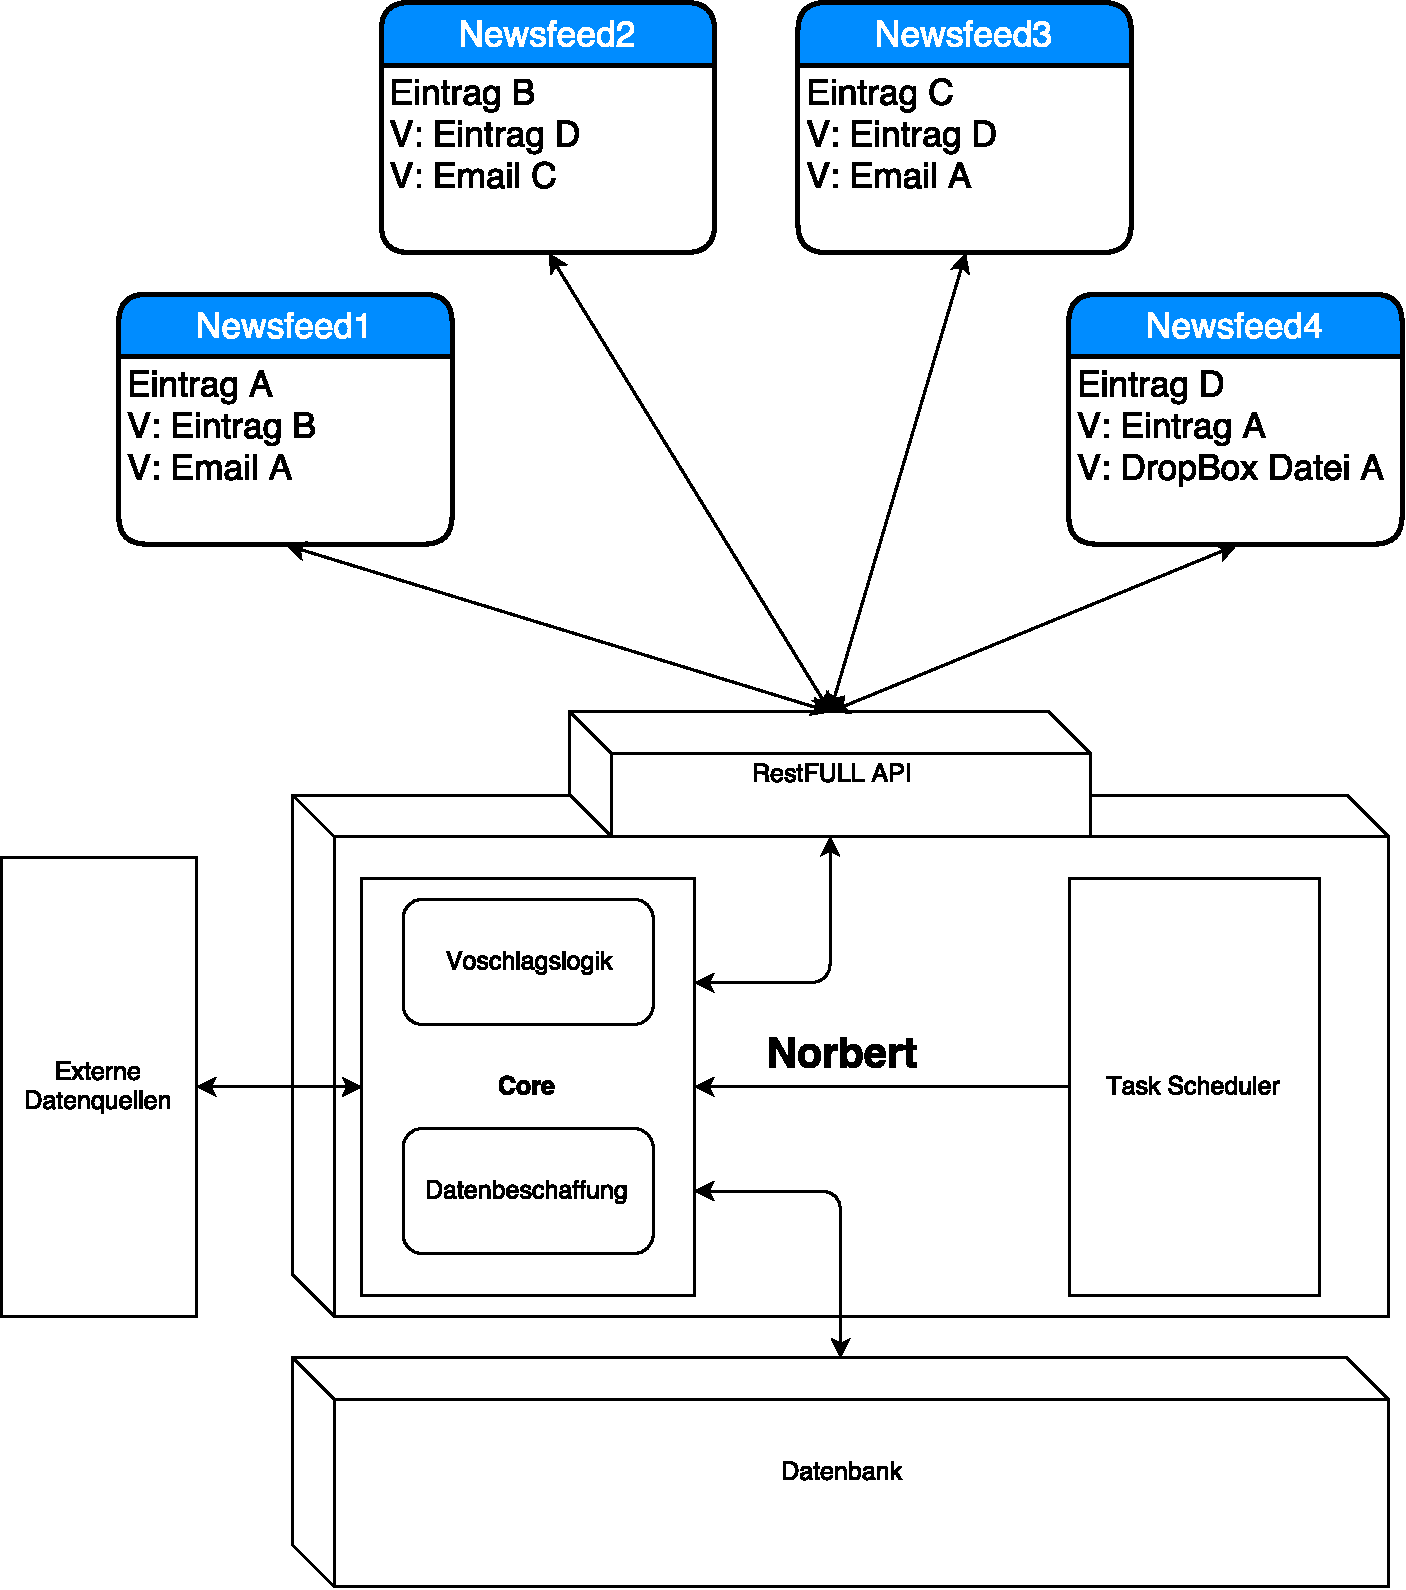
\includegraphics[scale=0.6]{uml-diagramms/overview_detail.pdf}
\caption{Kapselung der internen Prozesse}
\label{fig: Overview_Detail}
\end{figure}




        
